
\section{问题}
\subsection{挪亚洪水启示我们:神在审判之前先通知义人(挪亚)审判的消息。为什么主耶稣来到的日子要像夜间的贼?}
“主的日子来到好像夜间的贼"出自帖前5:1-8,“你们自己明明晓得,主的日子来到好像夜间的贼一样。人正说平安稳妥的时候,灾祸忽然临到\textcolor{blue}{他们},如同产难临到怀胎的妇人一样,\textcolor{blue}{他们}绝不能逃脱
。\textcolor{red}{弟兄们,你们},\textcolor{red}{你们}却不在黑暗里,叫那日子临到\textcolor{red}{你们}像贼一样。\textcolor{red}{你们}都是光明之子,都是白昼之子。\textcolor{red}{我们}不是属黑夜的,也不是属幽暗的。所以,\textcolor{red}{我们}不要睡觉,像别人一样,总要警醒谨守。 因为睡了的人是在夜间睡,醉了的人是在夜间醉。 但\textcolor{red}{我们}既然属乎白昼,就应当谨守,把信和爱当做护心镜遮胸,把得救的盼望当做头盔戴上"。
\setlist{nolistsep}
\begin{itemize}[noitemsep]
\item 对于“他们(不认识主的人)",主的日子来到确实好像夜间的贼一样
\begin{itemize}[noitemsep]
\item 主是忽然临到,因为主是在众人都说“平安稳妥的时候”来到。
\item 就如同睡觉的人在黑暗中看不清盗贼的脸一样,主耶稣的到来,“他们"也完全不知道。
\end{itemize}
\item 对于“你们/我们(光明之子)",只要我们警醒谨守,主的日子来到是在光明中
\end{itemize}

\subsection{我们将来所得的国度是虚拟(灵里)的,还是真实的在地上的?}
\begin{itemize}[noitemsep]
\item 我们现在得到的是属灵的福气:天上的耶路撒冷。
\begin{itemize}[noitemsep]
\item 加4:22-26 律法上記著,亞伯拉罕有兩個兒子,一個是使女生的,一個是自主之婦人生的。然而那使女所生的是按著血氣生的,那自主之婦人所生的是憑著應許生的。這都是比方:那兩個婦人就是兩約。一約是出於西奈山,生子為奴,乃是夏甲。這夏甲二字是指著阿拉伯的西奈山,與現在的耶路撒冷同類,因耶路撒冷和她的兒女都是為奴的。但那\underline{在上的耶路撒冷是自主的,她是我們的母}。
\item 彼前1:3 父神曾照自己的大憐憫,藉著耶穌基督從死裡復活重生了我們,叫我們有活潑的盼望,可以得著不能朽壞、不能玷汙、不能衰殘、為你們存留在\underline{天上的基業}。
\item 彼前2:4-5 主乃活石,固然是被人所棄的,卻是被神所揀選、所寶貴的。你們來到主面前,也就像\underline{活石},被建造\underline{成為靈宮},做聖潔的祭司,藉著耶穌基督奉獻神所悅納的靈祭。
\end{itemize}
\item 到主耶稣再来的时候,我们将承受神给亚伯拉罕的应许。\\
“你們因信基督耶穌,都是神的兒子。你們受洗歸入基督的,都是披戴基督了;並不分猶太人、希臘人,自主的、為奴的,或男或女,因為你們在基督耶穌裡都成為一了。你們\underline{既屬乎基督,就是亞伯拉罕的後裔,是照}\\
\underline{著應許承受產業的了(加4:26-29)}"。
\item 圣经中有许多关于千年国度的描述,列举部分供参考
\begin{itemize}[noitemsep]
\item 可能因为末后有许多地震,导致耶路撒冷成为世界上最高的山.\\
“末后的日子,耶和华殿的山必坚立超乎诸山,高举过于万岭,万民都要流归这山(賽2:2/彌4:1-3)。"
\item 以西结书40-48章提到,千年国度会重建圣殿,参考Figure 1(\ref{fig:sub1}\footnotetext{https://cmcbiblereading.com/wp-content/uploads/2021/09/Temple-Sizes-Comparison-1024x717.png})是以西结异象中的圣殿与摩西会幕、所罗门圣殿和希律圣殿的尺寸比较;并重新分配土地,参考Figure 2(\ref{fig:sub2}\footnotetext{https://cmcbiblereading.com/wp-content/uploads/2021/09/The-Sanctuary-Portion-1024x797.png})以色列「当献的供地」示意图。
\item 在那个时候,除了基督的国度,世界上还有其他的国家.这些战后得以进入千年国度的人们,每年7月15-22号都要来耶路撒冷过住棚节。\\
“所有來攻擊耶路撒冷列國中剩下的人,必年年上來敬拜大君王萬軍之耶和華,並守住棚節。地上萬族中,凡不上耶路撒冷敬拜大君王萬軍之耶和華的,必無雨降在他們的地上。埃及族若不上來,雨也不降在他們的地上。凡不上來守住棚節的列國人,耶和華也必用這災攻擊他們。這就是埃及的刑罰和那不上來守住棚節之列國的刑罰。當那日,馬的鈴鐺上必有「歸耶和華為聖的」這句話。耶和華殿內的鍋必如祭壇前的碗一樣。凡耶路撒冷和猶大的鍋都必歸萬軍之耶和華為聖,凡獻祭的都必來取這鍋,煮肉在其中。當那日,在萬軍之耶和華的殿中必不再有迦南人(撒迦利亞書14:16-20)。"
\end{itemize} 
\end{itemize}
%https://cmcbiblereading.com/wp-content/uploads/2021/09/The-Sanctuary-Portion-1024x797.png

\begin{figure} 
\centering
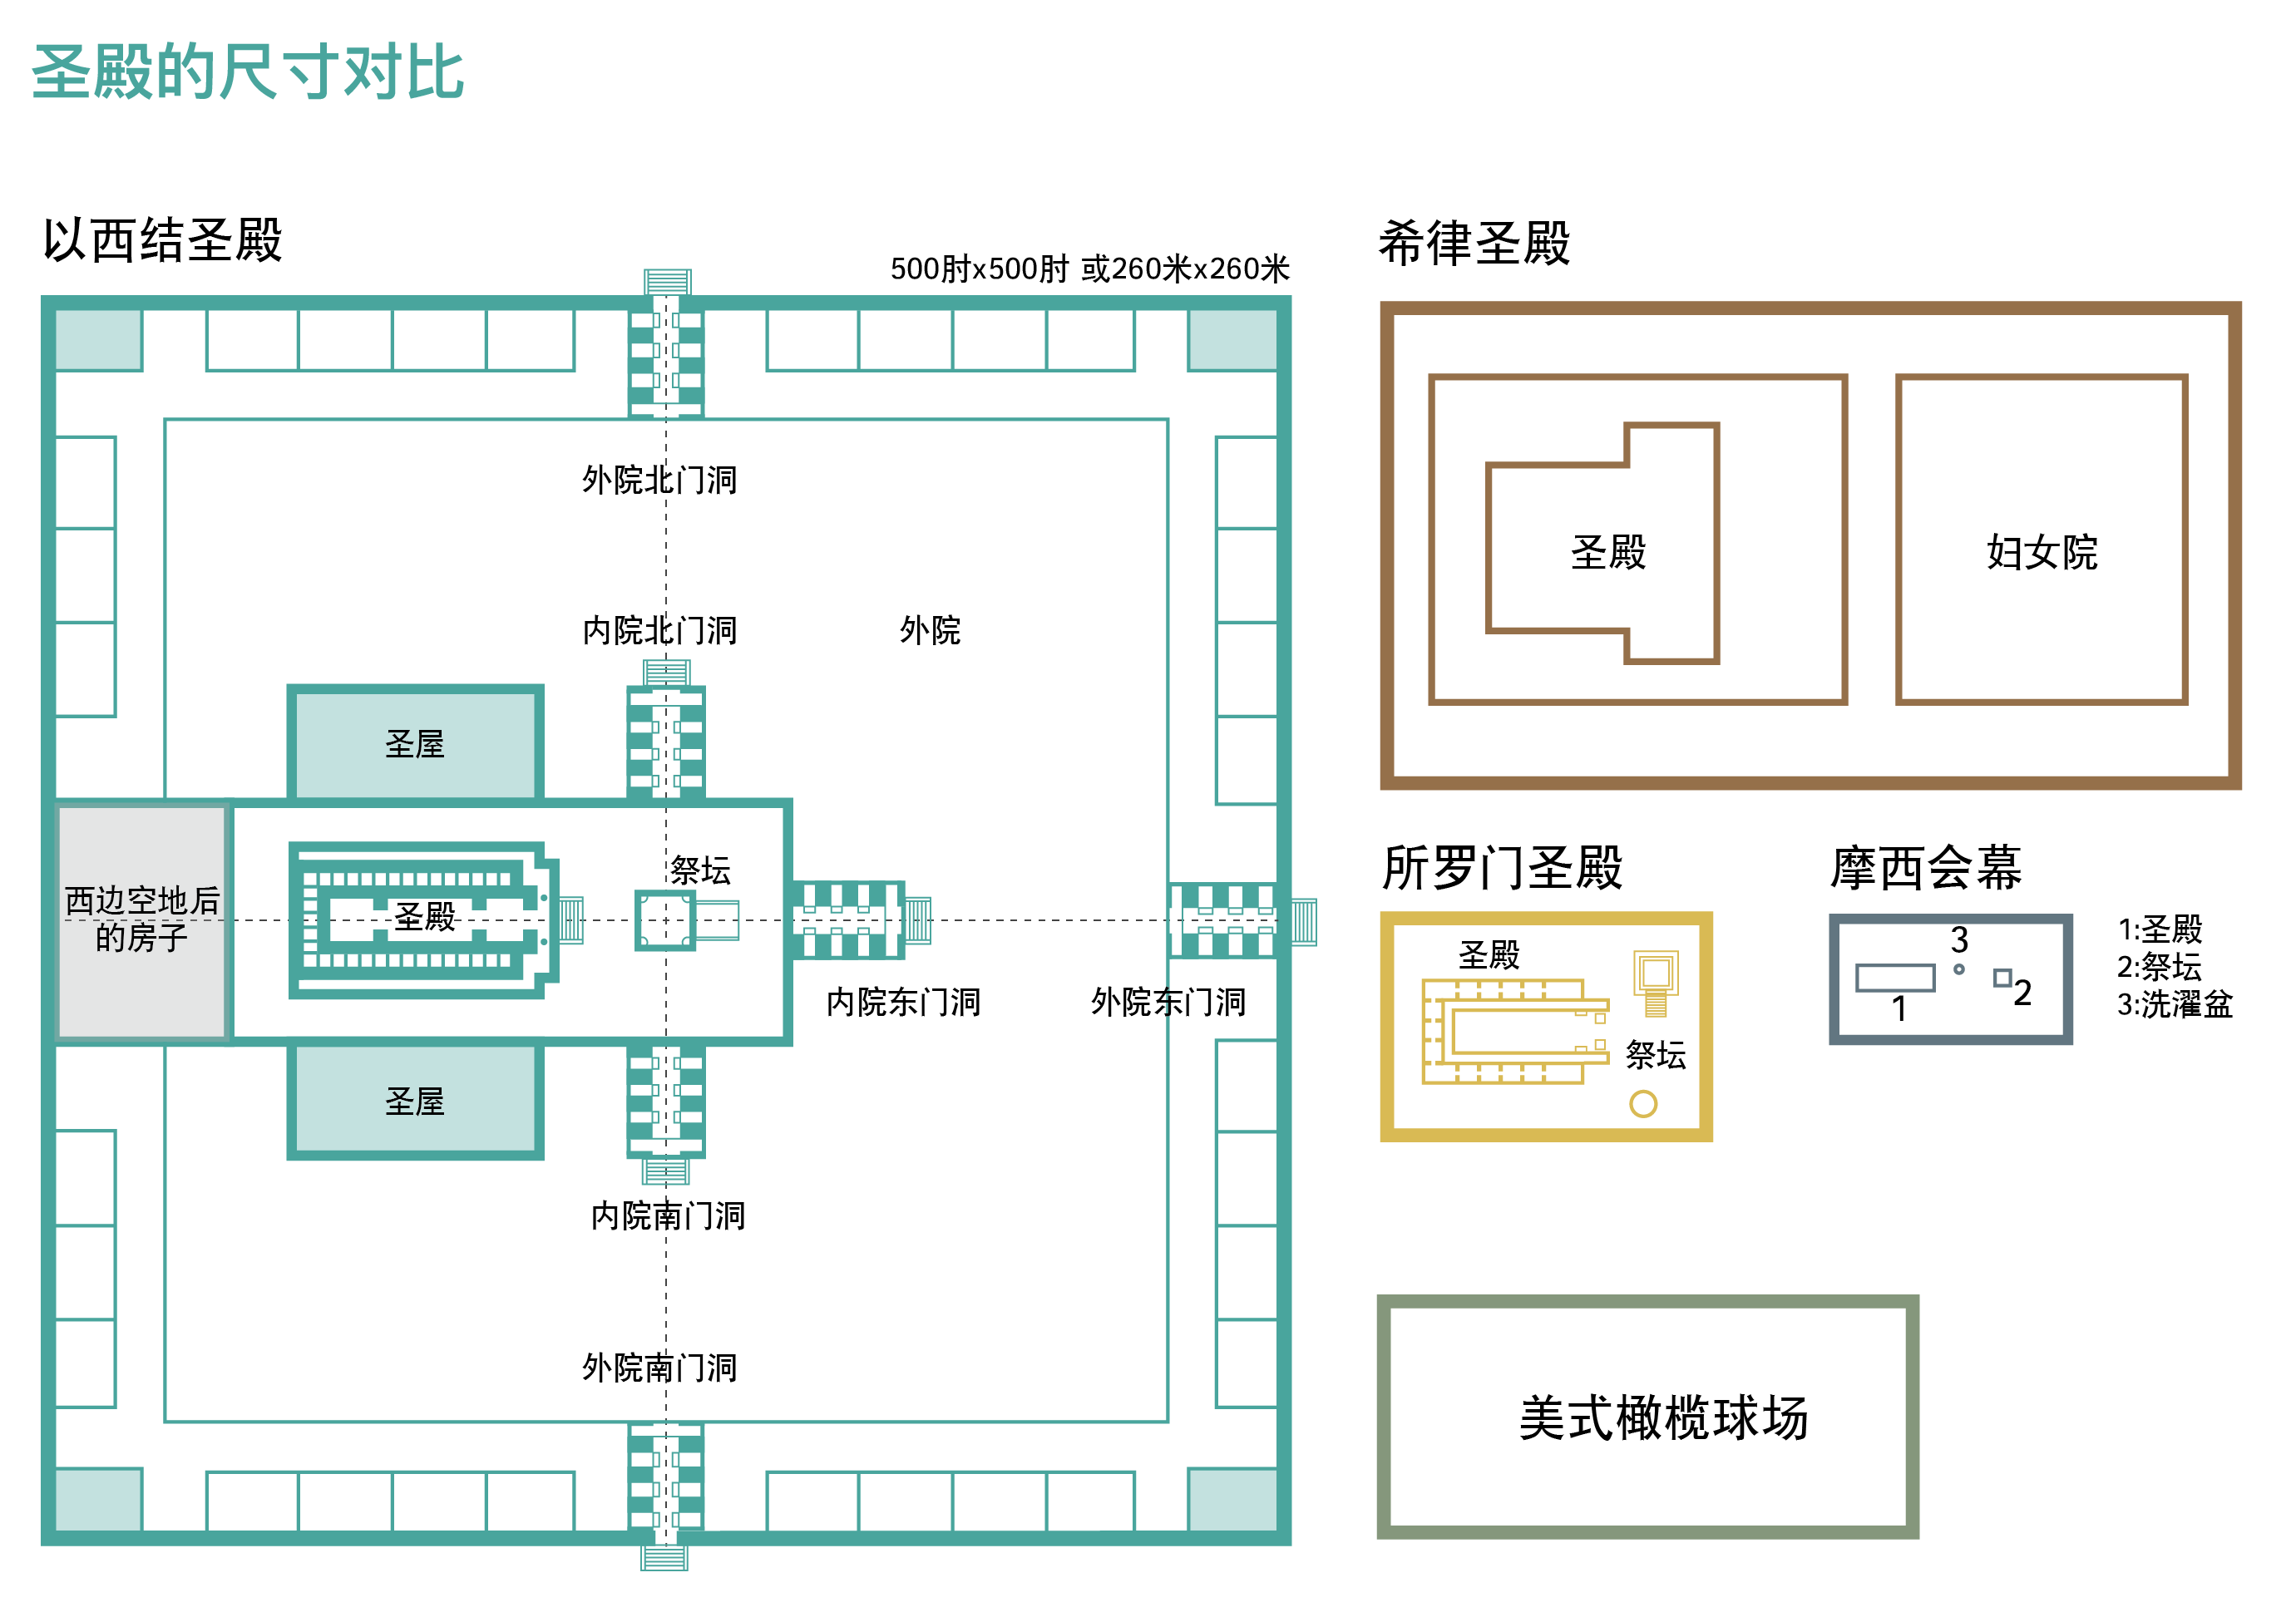
\includegraphics[width=5in]{TempleSizesComparison.png}
\caption{以西结异象中的圣殿与摩西会幕、所罗门圣殿和希律圣殿的尺寸比较}
\label{fig:sub1}
\end{figure} 

\begin{figure} 
\centering
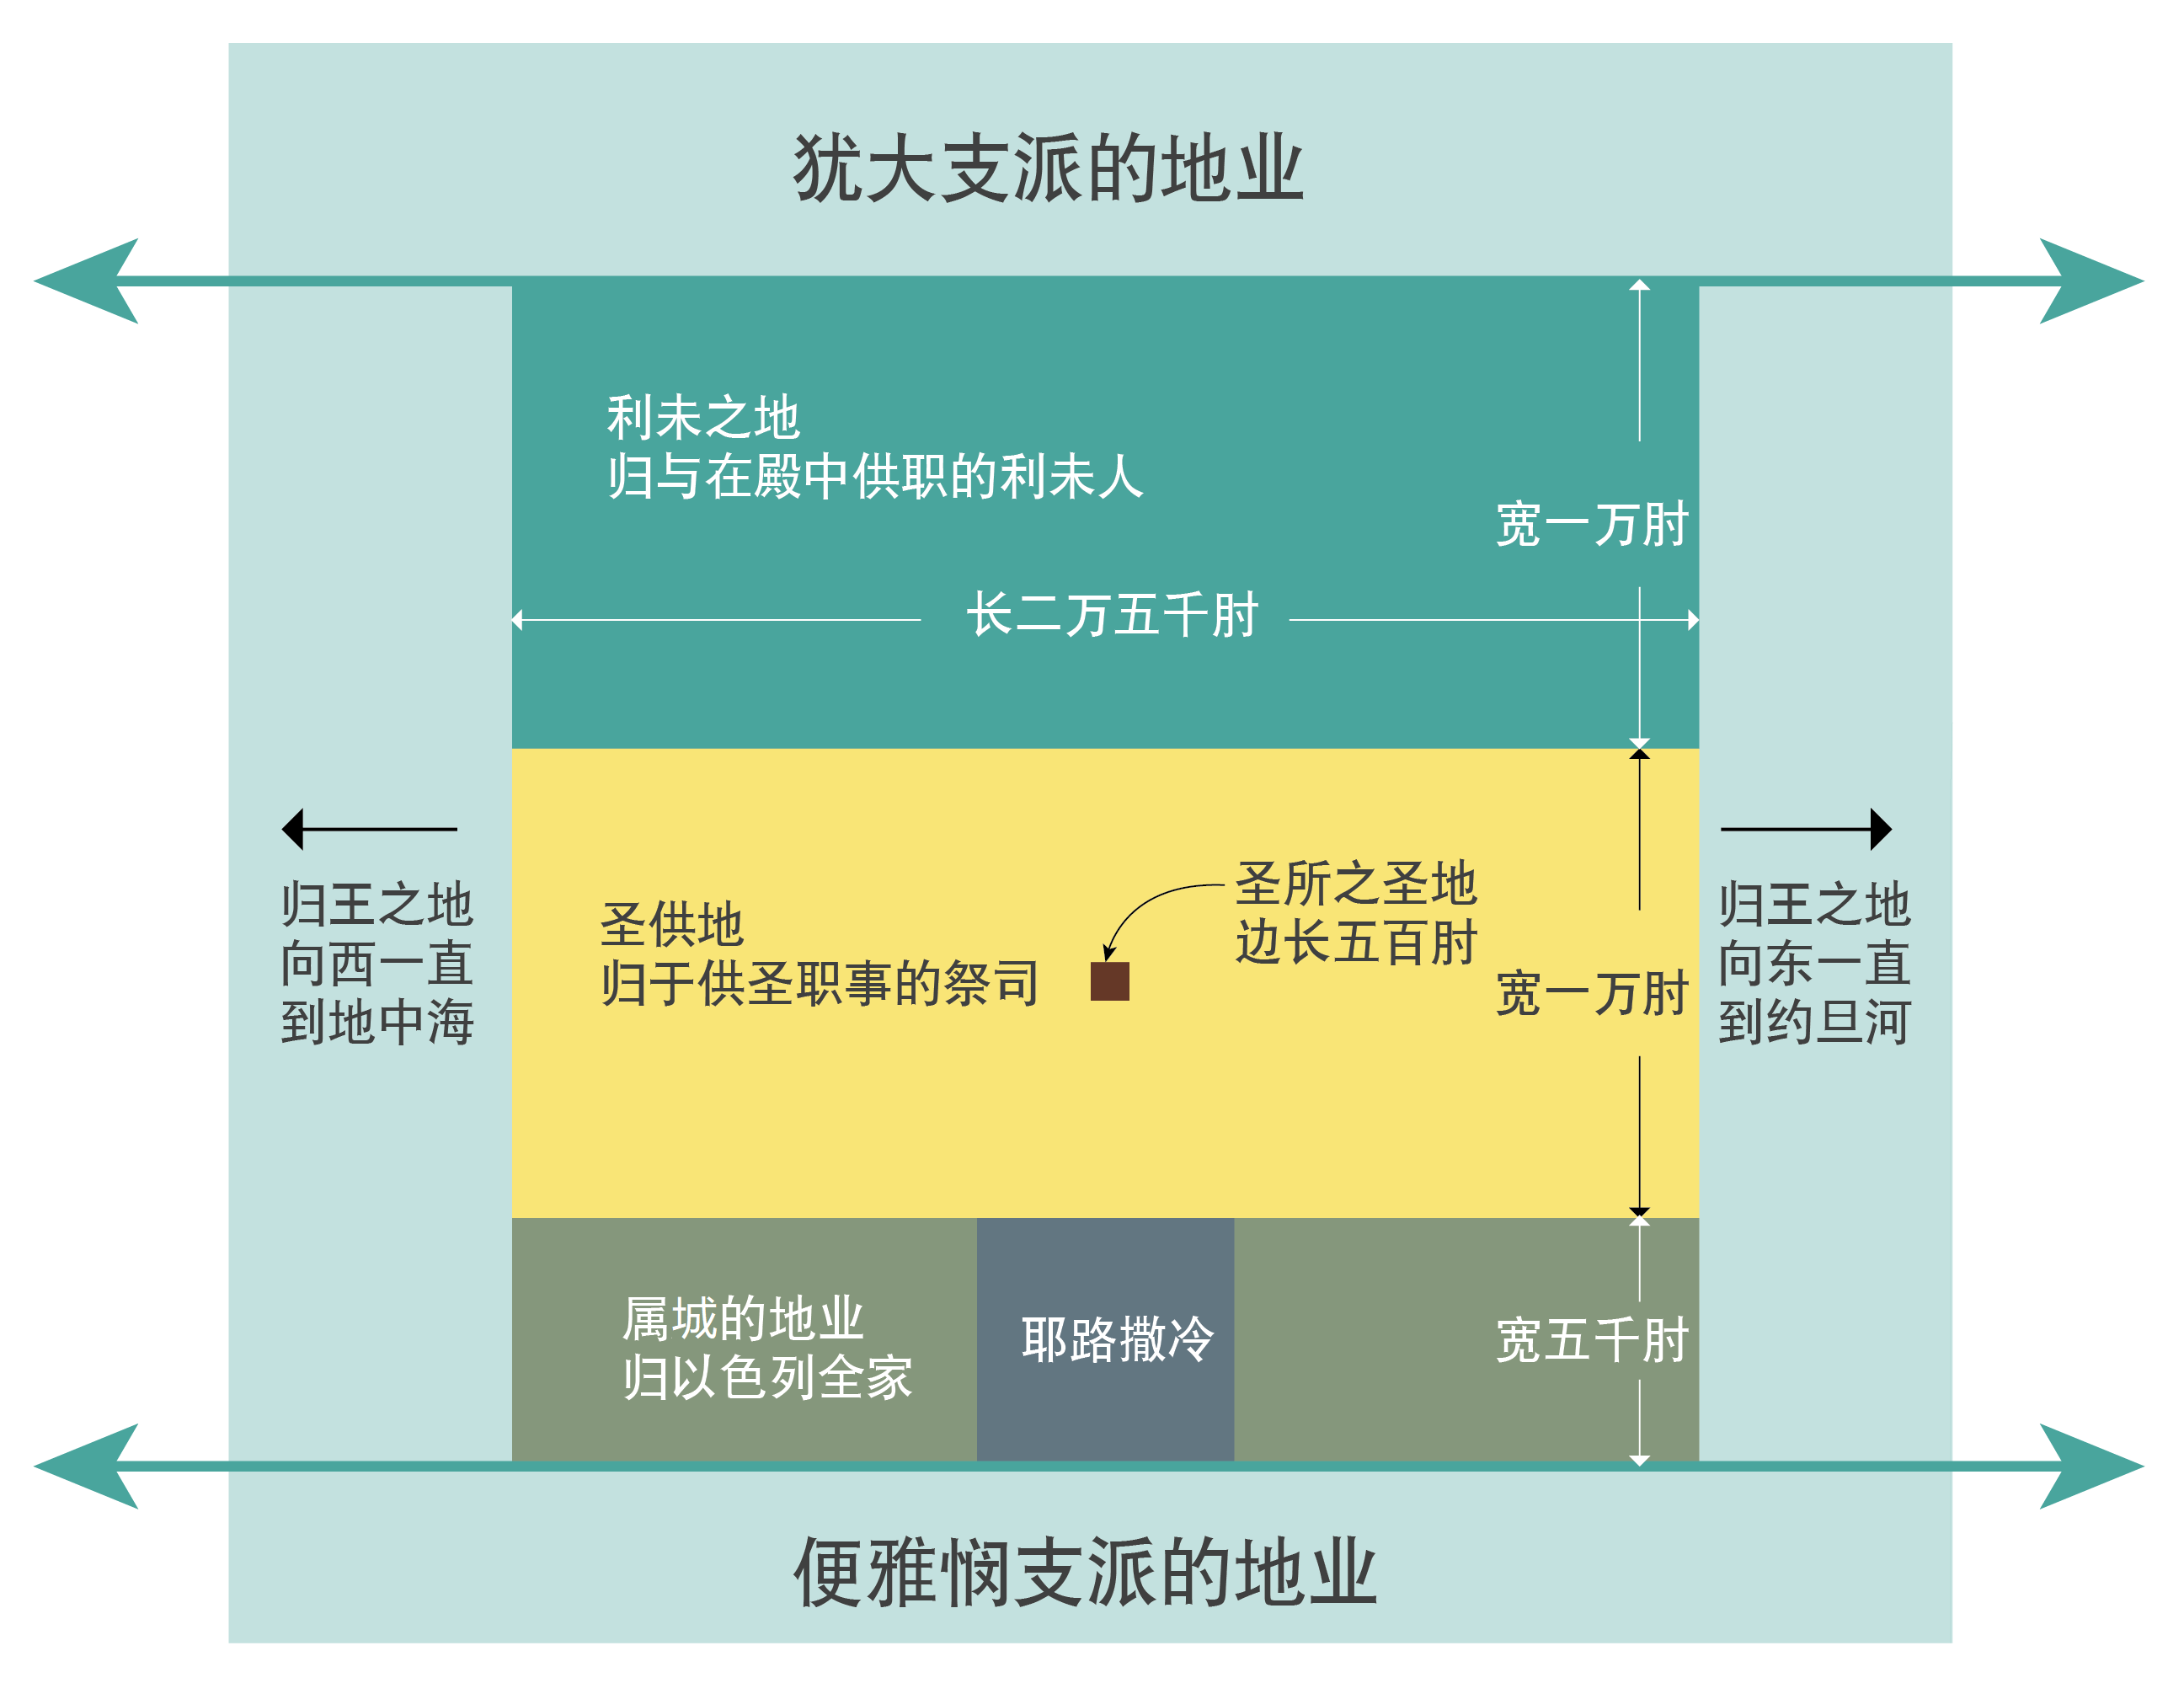
\includegraphics[width=5in]{land.png}
\caption{以西结异象里以色列「当献的供地」}
\label{fig:sub2}
\end{figure} 